%! TeX root = master.tex
% !TEX program = lualatex

\lecture{9}{21-04-2026}{Deep Learning (Part 1)}{}
\section{Deep Learning}
So far, all the representations we have used were manually designed. 
The key idea of neural networks is to \textbf{learn the representation 
jointly with the classifier}, removing the need for hand-crafted features. 
The model is built as a stack of \textbf{layers}, each composed of 
\textbf{neurons} connected to every neuron of the previous layer. Each 
neuron computes a weighted sum of its inputs, then passes the result 
through a \textbf{non-linear activation function} — without this 
non-linearity, the whole network would collapse into a single linear model. 
Depending on the output layer and the loss function used, the same 
architecture handles both \textbf{regression} (square loss) and 
\textbf{classification} (softmax + cross-entropy). This framework is 
referred to as \textit{neural network}, \textit{multilayer perceptron (MLP)}, 
or \textit{deep learning} when there are at least two hidden layers.\subsection{Parametric feature expansion}
As we have seen, parametric feature expansion isn't optimal as we need to define manually the polynomial expansion $\phi(x)$ and we would like to learn the representation conjointly with the classifier. 
To achieve this goal we have to add \textbf{nonlinearity} in the process. 

We will use a nonlinear function (\textbf{activation function}) $f: \mathbb{R} \to \mathbb{R}$.

\subsection{Hidden representation}

Let's first apply a linear transformation to the input (pre-activation) \[
  a_{(1)} = W_{(1)}^T \begin{pmatrix}
     1  \\
     x 
  \end{pmatrix} = \begin{pmatrix}
  W_{(1)}^{(1,0)} + W_{(1)}^{(1,1)}x   \\
  W_{(1)}^{(2,0)} + W_{(1)}^{(2,1)}x \\
  \vdots  \\
W_{(1)}^{(M,0)} + W_{(1)}^{(M,1)}x

  \end{pmatrix} = \begin{pmatrix}
  a_{(1)}^{(1)}  \\
  a_{(1)}^{(2)} \\
  \vdots  \\
a_{(1)}^{(M)}
  \end{pmatrix}
\]
Then we apply $f$ elementwise to $a_{(1)}$, and it gives our complete $M-$dimensional \textit{hidden representation} (analogous to a learn $\phi(x)$ of the feature expansion)\[
  x \to \begin{pmatrix}
    f(a_{(1)}^{(1)})   \\
  f(a_{(1)}^{(2)}) \\
    \vdots \\
    f(a_{(1)}^{(M)})
\end{pmatrix} = f \left(W_{(1)}^T \begin{pmatrix}
  1  \\
  x 
\end{pmatrix}\right) = z_{(1)} \in \mathbb{R}^M
\]
each of its $M$ elements is referred to as hidden unit.
\subsubsection{Complete model}
We can then perform prediction by applying a second linear
model to the hidden representation. 

This gives \[
  \hat{y} = w_{(2)}^T z_{(1)} = w_{(2)}^T f \left(W_{(1)}^T \begin{pmatrix}
    1  \\
    x 
\end{pmatrix}\right) = w_{(2)}^T \begin{pmatrix}
    f(a_{(1)}^{(1)})   \\
    f(a_{(1)}^{(2)}) \\
    \vdots \\
    f(a_{(1)}^{(M)})
\end{pmatrix}
= \sum_{j=1}^{M} w_{(2)}^{(j)} f \left(W_{(1)}^{(j,0)} + (W_{(1)}^{(j,1)}\right)
\]

And the resulting simple artificial neural network with one hidden
layer can be depicted as shown below. 

\begin{center} 
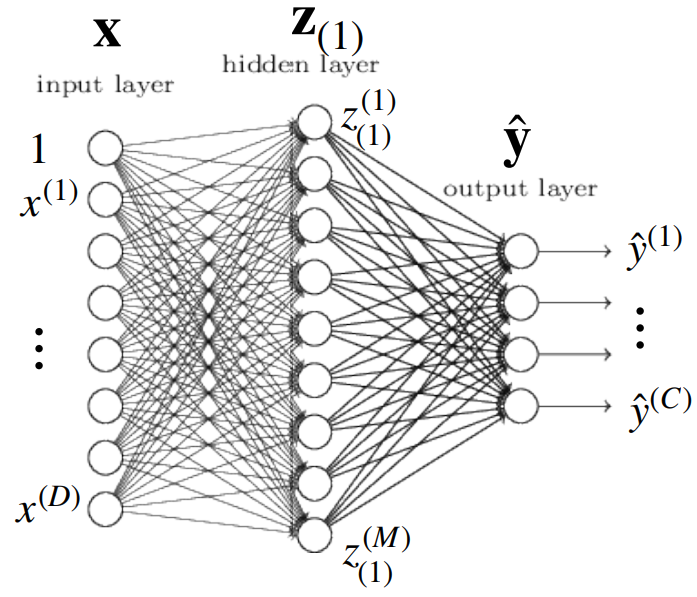
\includegraphics[width=0.4\linewidth]{images/img_20260421_120828.png}
\end{center}

Because we use a matrix-vector product for each layer, the layers are
called \textit{fully-connected} \begin{itemize}
  \item Each hidden dimension (hidden unit) $z_{(1)}^{(j)}$ depends on all input dimensions $x^{(1)}, ... x^{(D)}$   
  \item Each output dimension $\hat{y}^{(k)}$depends on all hidden units $z_{(1)}^{(1)}, ..., z_{(1)}^{(M)}$
\end{itemize}
In short, it means that each output neurons is connected to each input neurons.

\subsubsection{Extension to multi-dimensional input and output}
The formulation above assumed $x \in \mathbb{R}$ and $\hat{y} \in \mathbb{R}$. 
In the general case:
\begin{itemize}
  \item \textbf{Input} $x \in \mathbb{R}^D$: the bias is absorbed into $x$ 
  by appending a 1, so $W_{(1)} \in \mathbb{R}^{(D+1) \times M}$, and the 
  hidden representation becomes:
  \[
    z_{(1)} = f\!\left(W_{(1)}^T x\right)
  \]
  \item \textbf{Output} $\hat{y} \in \mathbb{R}^C$: we replace the vector 
  $w_{(2)}$ by a matrix $W_{(2)} \in \mathbb{R}^{M \times C}$, giving:
  \[
    \hat{y} = W_{(2)}^T z_{(1)} = W_{(2)}^T f\!\left(W_{(1)}^T x\right)
  \]
\end{itemize}
\subsubsection{Activation function: Examples}
\begin{itemize}
  \item Sigmoid: $f(a) = \frac{1}{1 + exp(-a)}$ 
  \item Hyperbolic tangent: $f(a) = tanh(a)$ 
  \item Rectified Linear Unit (ReLU) \[
    f(a) = \begin{cases}
      a & \text{if } a > 0 \\ 0 & \text{otherwise} \end{cases} = \max(a, 0)
    \end{cases}
  \]
\end{itemize}
\begin{center}
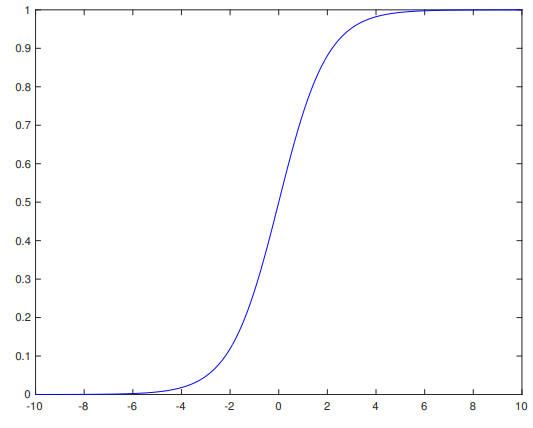
\includegraphics[width=0.25\linewidth]{images/img_20260421_114300.png}
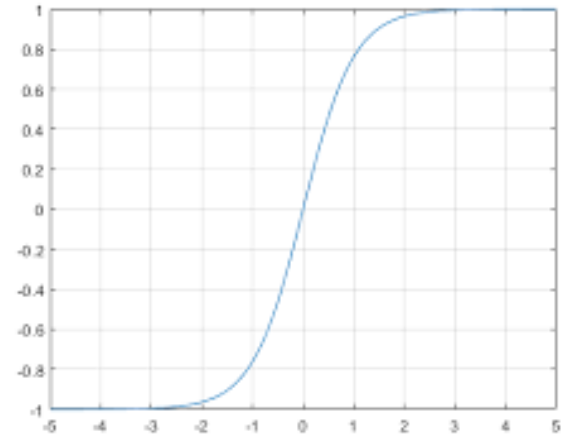
\includegraphics[width=0.25\linewidth]{images/img_20260421_114307.png}
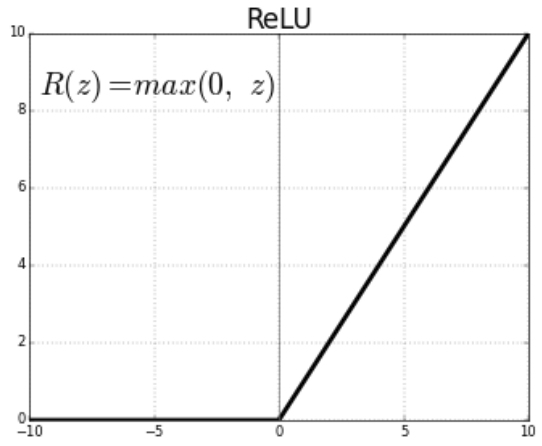
\includegraphics[width=0.25\linewidth]{images/img_20260421_114319.png}
\end{center}
\subsection{Multilayer Perceptron (MLP)}
\subsubsection{Architecture}
With a single hidden layer we can already model complicated functions, 
but we can stack multiple layers. 

In essence, each hidden layer takes as input the output of the previous layer.

For the first hidden layer ():
\[
  z_{(1)} = f\left(W_{(1)}^T x\right)
\]
For any subsequent layer $l$:
\[
  z_{(l)} = f\left(W_{(l)}^T z_{(l-1)}\right)
\]
For a network of $L$ layers, the output is:
\[
  \hat{y} = W_{(L)}^T z_{(L-1)}
\]
This process of going from input to output is called the \textbf{forward pass}.
We can write the prediction as a function of all parameters $W = \{W_{(l)}\}$:
\[
  \hat{y} = W_{(L)}^T f\left(W_{(L-1)}^T f\left(W_{(L-2)}^T f\left(\cdots f\left(W_{(1)}^T x\right)\cdots\right)\right)\right) = \hat{y}(W)
\]
As we have seen with the $1D$ example, because we use a matrix-vector product at each layer, the layers are called 
\textbf{fully-connected}: each hidden unit $z_{(l)}^{(j)}$ depends on all units 
of the previous layer.

\subsubsection{Universal approximation}
Any continuous function can be approximated by a linear combination of 
translated and scaled activation functions. This holds for ReLU and other 
activation functions under mild assumptions.

\subsection{Training an MLP}
\subsubsection{Empirical risk minimization}
Training is done by minimizing an empirical risk over all parameters $W$:
\[
  R(W) = \frac{1}{N} \sum_{i=1}^{N} \ell(\hat{y}_i(W), y_i)
\]
For regression, the typical loss is the \textbf{square loss}:
\[
  R(W) = \frac{1}{N} \sum_{i=1}^{N} \|\hat{y}_i(W) - y_i\|^2
\]
Since the problem is non-convex and has no closed-form solution, 
learning is done by \textbf{gradient descent}.

\subsubsection{Backpropagation}
Because the empirical risk is an average over the training
samples, its gradient will also be an average of gradients. 

Thus we can focus on a single loss term $\ell_i = \ell(\hat{y}_i, y_i)$ where \[
  R(W_{\ell}) = \frac{1}{N} \sum_{i=1}^{N} \ell(\hat{y}_i(W), y_i) = \frac{1}{N}\sum_{i=1}^{N} \ell_i
\]
For the $k$-th dimension of the output of any layer $l$, let us define the pre-activation:
\[
  a_{(l)}^{(k)} = \sum_j W_{(l)}^{(k,j)} z_{(l-1)}^{(j)}
\] which denotes the dot product between the $k^{th}$ column of $W_{(l)}$ and $z_{(l-1)}$.

What we aim to compute is the derivative of the loss function $\ell_i$ w.r.t. any parameter $W_{(l)}^{(k,j)}$

By the chain rule:
\[
  \frac{\partial \ell_i}{\partial W_{(l)}^{(k,j)}} = 
  \underbrace{\frac{\partial \ell_i}{\partial a_{(l)}^{(k)}}}_{\delta_{(l)}^{(k)}} 
  \cdot \underbrace{\frac{\partial a_{(l)}^{(k)}}{\partial W_{(l)}^{(k,j)}}}_{z_{(l-1)}^{(j)}}
\]
Defining $\delta_{(l)}^{(k)} = \frac{\partial \ell_i}{\partial a_{(l)}^{(k)}}$, we get:
\[
  \frac{\partial \ell_i}{\partial W_{(l)}^{(k,j)}} = \delta_{(l)}^{(k)} \cdot z_{(l-1)}^{(j)}
\]
For the last layer $L$ (square loss, no final activation):
\[
  \delta_{(L)}^{(k)} = 2(\hat{y}_i^{(k)} - y_i^{(k)})
\]
For earlier layers $l < L$, $\delta_{(l)}$ is computed from $\{\delta_{(l+1)}^{(j)}\}$, 
$W_{(l+1)}$, and $f'$. 

In other words, given $\delta_{(l + 1)}$, we can compute $\delta_{(l)}$. So because we can explicitly compute $\delta_{(L)}$ for the last layer, we can in turn compute any $\delta_{(l)}$.

This gives us a way to compute the gradient at any layer, starting from the last one and it's called the \textbf{backpropagation} algorithm:
\begin{enumerate}
  \item Propagate $x_i$ forward through the network and at each layer compute and store $z_{(1)}, \dots, z_{(L-1)}$
  \item Compute $\delta_{(L)}$ from the loss
  \item Propagate $\delta_{(L)} $backward to obtain each $\delta_{(l)}$
  \item At each layer, compute $\frac{\partial \ell_i}{\partial W_{(l)}^{(k,j)}} = \delta_{(l)}^{(k)} z_{(l-1)}^{(j)}$

    where $z_{l-1}$ has been computed during the forward pass.
\end{enumerate}

\\
So the training consists of repeating this until convergence: 
\begin{enumerate}
  \item \textbf{Forward pass : } propagate $x_i$ through each layer to compute and $z_{(l)}$ 
  \item \textbf{Backpropagation : } compute each $\delta_{(l)}$, starting from the last layer, and gives us the gradient $\frac{\partial \ell_i}{\partial W_{(l)}^{(k,j)}}$ 
  \item \textbf{Gradient descent : } use those gradients to update the weights $W_i$
\end{enumerate}

\subsection{Optimization}
\subsubsection{Gradient descent and SGD}
The standard gradient descent update at iteration $k$:
\[
  W_k \leftarrow W_{k-1} - \eta \frac{1}{N}\sum_{i=1}^{N} \nabla_W \ell_i(W_{k-1})
\]
This is expensive for large $N$. 

\textbf{Stochastic gradient descent (SGD)} 
uses a single sample per iteration:
\[
  W_k \leftarrow W_{k-1} - \eta \nabla \ell_{i(k)}(W_{k-1})
\]
But as the gradient obtained by a single sample might be a poor approximation of the true, complete gradient, we use mini-batches $B$ samples for a more reliable gradient estimate:
\[
  W_k \leftarrow W_{k-1} - \eta \sum_{b=1}^{B} \nabla \ell_{i(b,k)}(W_{k-1})
\]
SGD introduces noise in the updates, which can help escape bad local minima, 
but causes oscillations that may require decreasing $\eta$.
\begin{center}
   
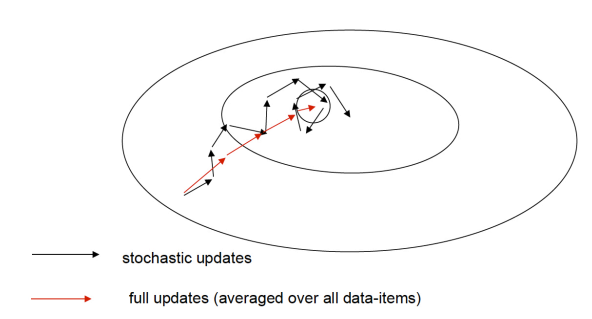
\includegraphics[width=0.5\linewidth]{images/img_20260421_140001.png}
\end{center}

\subsubsection{SGD extensions}
\paragraph{Momentum} Adds inertia to the parameter updates:
\[
  \nu \leftarrow \gamma\nu + \eta \nabla R(W), \qquad W \leftarrow W - \nu
\]
with $\gamma > 0$, momentum 
\begin{itemize}
  \item Accelerates if the gradient does not change too much 
  \item Dampens (slow down) the oscillations in narrow valleys
\end{itemize}
\begin{center}
   
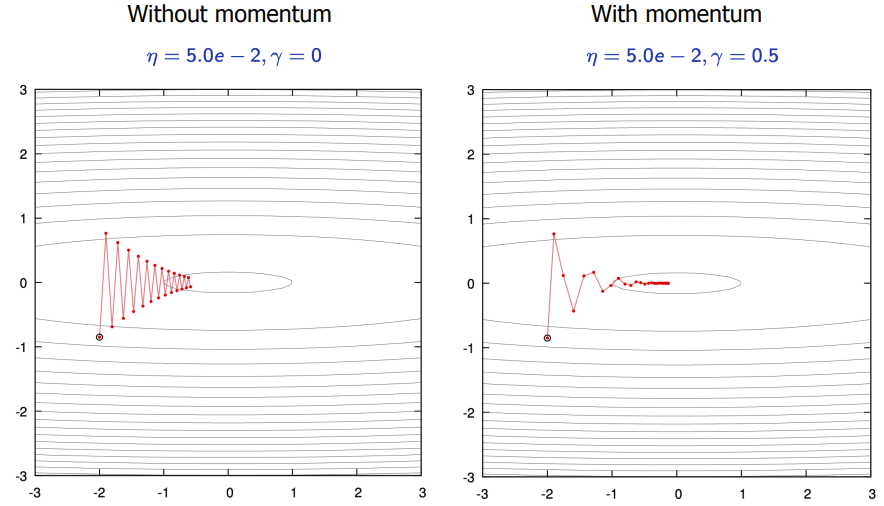
\includegraphics[width=0.5\linewidth]{images/img_20260421_140907.png}
\end{center}


\paragraph{Adaptive learning rate} Methods such as \textbf{ADAM} 
(Kingma et al., ICLR 2015) maintain a moving average per coordinate 
to rescale each dimension of the gradient separately. 
\begin{center}  
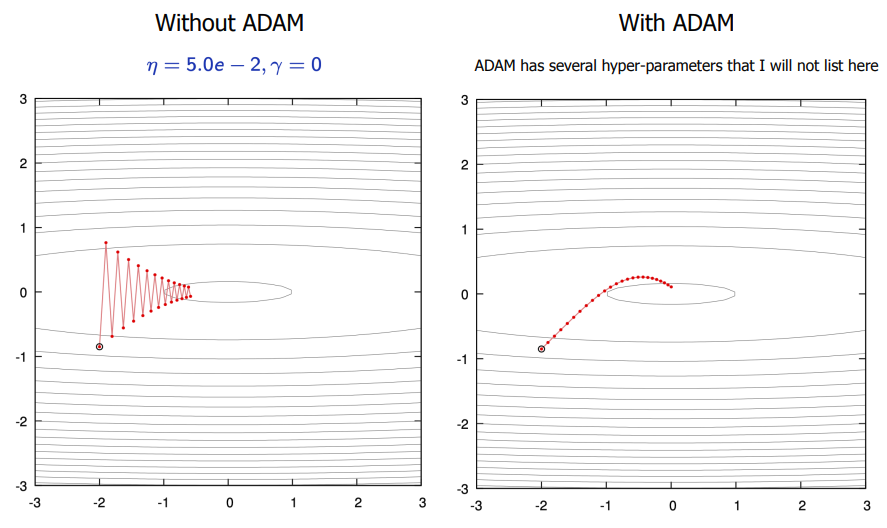
\includegraphics[width=0.5\linewidth]{images/img_20260421_141043.png}
\end{center}

\subsection{Practical training issues}
\subsubsection{Gradient vanishing and initialization}
The \textbf{vanishing gradient} problem arises when backpropagating through 
deep networks: at each layer, the gradient is multiplied by $f'(a)$, the 
derivative of the activation function. Since sigmoid and tanh saturate for 
large $|a|$, their derivative becomes close to 0 in these regions. With poor 
weight initialization, activations tend to fall in these saturating regions, 
causing the gradient to shrink exponentially as it propagates back through 
the layers — meaning the first layers receive almost no learning signal. 

To overcome this we could use \textit{Xavier (Glorot) initialization}: a weight initialization strategy where the range of the initial, random
values of the weights is layer dependent. 
\begin{center}
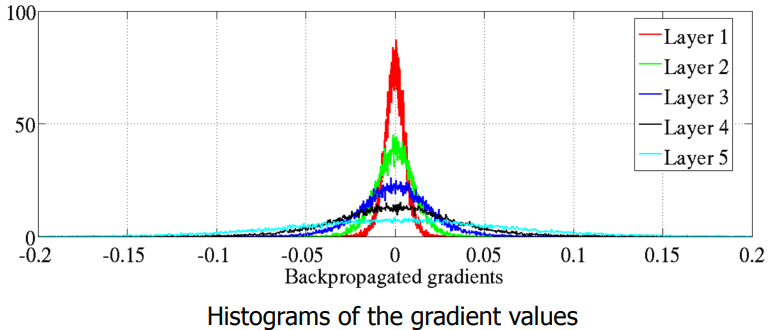
\includegraphics[width=0.49\linewidth]{images/img_20260421_141737.png}
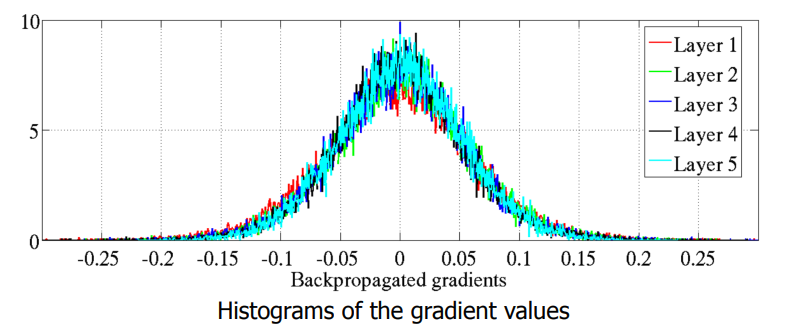
\includegraphics[width=0.49\linewidth]{images/img_20260421_142224.png}
\end{center}

\subsubsection{Regularization}
Deep networks have many parameters and can overfit. Solutions include:
\begin{itemize}
  \item $L_1$ / $L_2$ regularization (seen previously)
  \item \textbf{Dropout} (Srivastava et al., JMLR 2014): randomly remove 
  units and their connections during training
\end{itemize}

\subsection{From regression to classification}
For classification, the output layer uses the \textbf{softmax} function 
to produce class probabilities:
\[
  \hat{y}^{(k)} = \frac{\exp\!\left(w_{(L)(k)}^T z_{(L-1)}\right)}
  {\sum_{j=1}^{C} \exp\!\left(w_{(L)(j)}^T z_{(L-1)}\right)}
\] where $w_{(L)(j)}$ indicates the $j^{th}$ column of $W_{(L)}$. 

The empirical risk is then the \textbf{cross-entropy}:
\[
  R(W) = -\frac{1}{N} \sum_{i=1}^{N} \sum_{k=1}^{C} y_i^{(k)} \ln \hat{y}_i^{(k)}
\]

And the backpropagation then requires computing the derivative of
the cross-entropy w.r.t each $\hat{y}^{(y)}$ and the derivative of the softmax function w.r.t each $W_{(L)}^{(j,k)}$.
